\section{Durchführung}
\label{sec:Durchführung}
Verwendet wird die in Abbildung \ref{fig:schaltung2} dargestellte Schaltung. Zu Beginn wird der
Selektivverstärker untersucht. Dieser ist nötig, da bei Brückenschaltungen Störspannungen auftreten.
Damit die zu messende Brückenspannung nicht von dieser Störung überdeckt wird, wird ein
Selektivverstärker eingesetzt, welcher die Störspannung herausfiltert und die Brückenspannung
verstärkt. Um die Frequenz zu bestimmen, welche der Selektivverstärker verstärkt, wird ein
Synthesizer angeschlossen. Mit ihm lässt sich die Frequenz $\nu$ variieren. Die Ausgangsspannung
$U_\text{A}$ wird über einen Bereich von ca. $(20-40)\,\si{\kilo\hertz}$ gemessen.

\noindent Zur Messung der Suszeptibilität $\chi$ wird zunächst die Speisespannung $U_\text{Sp}$
notiert. Anschließend wird die Brücke abgeglichen. Die Einstellung des Abgleichelements, sowie die
Brückenspannung $U_\text{Br}$ werden notiert. Eine Probe wird in eine der beiden Spulen eingeführt.
Die neue Brückenspannung wird gemessen. Anschließend wird die Brücke wieder abgeglichen und die
Einstellung des variablen Widerstands wird festgehalten. Diese Messung wird für jede der zu
untersuchenden Proben drei Mal durchgeführt.

\begin{figure}[H]
\centering
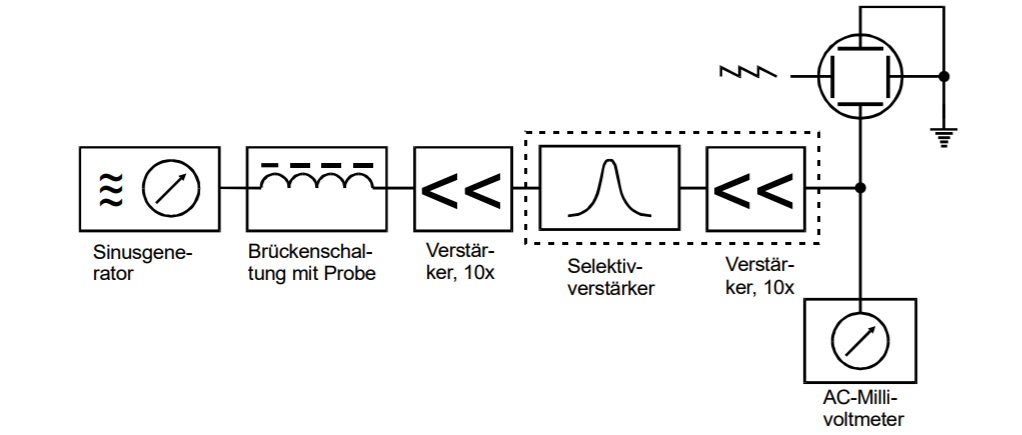
\includegraphics[scale=0.8]{schaltung2.png}
\caption{Schaltung zur Suszeptibilitätsmessung \cite{kent}.}
\label{fig:schaltung2}
\end{figure}
